% !TeX program = xelatex
% !TeX options = -shell-escape
% !TEX encoding = UTF-8

% --------------------------------------------------------------
% This is all preamble stuff that you don't have to worry about.
% Head down to where it says "Start here"
% --------------------------------------------------------------

\documentclass[12pt]{article}
\usepackage[margin=2cm]{geometry} % 頁面邊距設置
\usepackage{amsmath,amssymb,amsthm} % 數學相關套件
\usepackage{graphicx} % 圖形插入
\usepackage{booktabs} % 表格線條
\usepackage[AutoFakeBold,AutoFakeSlant]{xeCJK} % 中文支援
\usepackage{fancyhdr} % 頁首頁尾設置
\usepackage{xcolor,changepage,mdframed} % 顏色與框線相關
\usepackage{titlesec} % 標題格式
\usepackage{setspace} % 行距
\usepackage{tabularx}
\usepackage{minted} % 程式碼高亮（需安裝 Python 套件 pygments）
\usepackage[shortlabels]{enumitem} % 列表格式
\usepackage[colorlinks=true,linkcolor=black,urlcolor=blue,citecolor=blue]{hyperref}
% 超連結
\graphicspath{{images}}

% 字體設定 (xeCJK)
\setCJKmainfont{黑體-繁}
\setCJKmonofont{Noto Sans CJK TC}

% 頁首/頁尾設定 (fancyhdr)
\pagestyle{fancy}
\fancyhead[L]{NASA Homework 4} % 可以用 \leftmark 取代
\fancyhead[R]{B13901011 吳亞倫}
\fancyfoot[C]{\thepage}
\renewcommand{\headrulewidth}{0.4pt}
\renewcommand{\footrulewidth}{0pt}
\setlength{\headheight}{15pt}

% tex-fmt: off
\newtheorem*{theorem}{Theorem}
\newenvironment{lemma}[2][Lemma]{\begin{trivlist}
\item[\hskip \labelsep {\bfseries #1}\hskip \labelsep {\bfseries #2.}]}{\end{trivlist}}
\newenvironment{exercise}[2][Exercise]{\begin{trivlist}
\item[\hskip \labelsep {\bfseries #1}\hskip \labelsep {\bfseries #2.}]}{\end{trivlist}}
\newenvironment{problem}[2][Problem]{\begin{trivlist}
\item[\hskip \labelsep {\bfseries #1}\hskip \labelsep {\bfseries #2}]}{\end{trivlist}}
\newenvironment{question}[2][Question]{\begin{trivlist}
\item[\hskip \labelsep {\bfseries #1}\hskip \labelsep {\bfseries #2.}]}{\end{trivlist}}
\newenvironment{corollary}[2][Corollary]{\begin{trivlist}
\item[\hskip \labelsep {\bfseries #1}\hskip \labelsep {\bfseries #2.}]}{\end{trivlist}}
\newenvironment{solution}{\begin{proof}[Solution]}{\end{proof}}
\newenvironment{answer}{\begin{proof}[Ans]}{\end{proof}}

% 樣式設定

\setminted{frame=lines, linenos, framesep=2mm, breaklines=true, breakanywhere=true, autogobble=true}

% 自訂框線環境
\newmdenv[
  linewidth=2pt, linecolor=gray, backgroundcolor=gray!10,
  topline=false, bottomline=false, rightline=false,
  skipabove=10pt, skipbelow=10pt, innerleftmargin=10pt,
  innerrightmargin=0pt, innertopmargin=5pt, innerbottommargin=5pt
]{myquote}

\newenvironment{mycolorbox}[1][gray]{
  \renewmdenv[
    linewidth=2pt, linecolor=#1, backgroundcolor=#1!10,
    topline=false, bottomline=false, rightline=false,
    skipabove=10pt, skipbelow=10pt, innerleftmargin=10pt,
    innerrightmargin=0pt, innertopmargin=5pt, innerbottommargin=5pt
  ]{myquote}
  \begin{myquote}
}{\end{myquote}}

\linespread{1.1}
% \usemintedstyle{xcode}
\AtBeginEnvironment{minted}{\vspace{-10pt}} % 可根據需求調整間距數值
\setminted{breaklines=true, breakanywhere=true, autogobble=true}

% tex-fmt: on
\begin{document}
\thispagestyle{fancy}

%------------------------------------------------------------
%                         Start here
% -----------------------------------------------------------

\begin{center}
  {\large \bfseries Network Administration / System Administration} \\
  \vspace{1em}
  {\Large \bfseries Homework 4} \\
\end{center}

\vspace{2em}

\begin{tabular}{@{}l l}
  \textbf{Student:} & 吳亞倫 \\
  \textbf{ID:} & B13901011  \\
  \textbf{Department:} & 電機工程學系
\end{tabular}
\bigskip

\begin{mycolorbox}[cyan]
  \textbf{Discussion Partners:}
  \begin{itemize}
    \item Classmates：賴泓安、鄭竣陽、喻慈恩
      \vspace{0.5em}
  \end{itemize}
\end{mycolorbox}

\section{Short Answer}

\begin{mycolorbox}[teal]
  \textbf{Reference:}
  \footnotesize
  \begin{enumerate}
    \item \url{https://docs.opnsense.org/manual/firewall.html#action}
    \item \url{https://docs.opnsense.org/manual/firewall.html#direction}
    \item
      \url{https://docs.opnsense.org/manual/firewall_generic.html#address-types}
  \end{enumerate}
\end{mycolorbox}

\begin{enumerate}
  \item Block 會直接把封包丟掉，並且不會通知 Client 端他被 Block 了。通常用在不被信任的網路當中。而 Reject 則會通知 Client 此封包被拒絕接受，在 TCP 當中會回傳 RST 封包，而在 UDP 當中會回傳 ICMP Port Unreachable 封包。此設定多半用在可被信任的網路或是內部網路當中。

  \item In(comming) 代表的是封包從 Source 進入到防火牆時要進行防火牆規則的審查，而 Out(going) 代表的是封包從防火牆出去到 Destination 時再審查。通常預設都是使用 In 來設定防火牆規則。

  \item Network 指的是分配給該 interface 的所有網路，包含被 assign 的虛擬 IP 位址。而 Address 指的是所有該 interface 上的 IP 位址。一般常見的設定當中，都是選擇 interface network。
\end{enumerate}

\section{OPNsense}
\begin{mycolorbox}[teal]
  \textbf{Reference:}
  \footnotesize
  \begin{itemize}
    \item \url{https://docs.opnsense.org/manual/install.html} (Problem 2.1)
    \item \href{https://www.zenarmor.com/docs/network-security-tutorials/how-to-setup-dhcp-server-on-opnsense/}{How to Setup DHCP Server on OPNsense} (Problem 2.3)
    \item \url{https://docs.opnsense.org/manual/aliases.html} (Problem 2.4)
    \item \url{https://docs.opnsense.org/manual/settingsmenu.html#secure-shell} (Problem 2.5)
    \item \url{https://docs.opnsense.org/manual/aliases.html#url-tables} (Problem 2.6)
    \item \href{https://www.allthingstech.ch/using-opnsense-and-ip-blocklists-to-block-malicious-traffic/}{Using OPNsense and IP Blocklists to Block Malicious Traffic} (Problem 2.6)
    \item \href{https://www.provya.com/blog/opnsense-time-based-rules/}{OPNsense Time Based Rules} (Problem 2.6)
  \end{itemize}
\end{mycolorbox}

% Problem 2.1
\subsection{}
\begin{enumerate}
  \item 根據 Lab 5 的方法，在 VirtualBox 當中新增一台 OPNsense 虛擬機，設定如下：
    \begin{itemize}
      \item CPU：1 Core
      \item Memory： 4 GB
      \item Storage： 16 GB
      \item Network Adapter 1: Host-only Adapter
      \item Network Adapter 2: NAT Network
      \item Installation Media: OPNsense-25.1-dvd-amd64.iso
    \end{itemize}
  \item 以 \texttt{installer / opnsense} 登入。
  \item 點選 Install (ZFS) 進行安裝，之後點選 \texttt{stripe}，在硬碟選擇時選擇 \texttt{ada0} 進行安裝。
  \item 安裝完成後，會跳出設定 Root Password 的畫面，輸入學號完畢後按下 Enter。
    \begin{figure}[H]
      \centering
      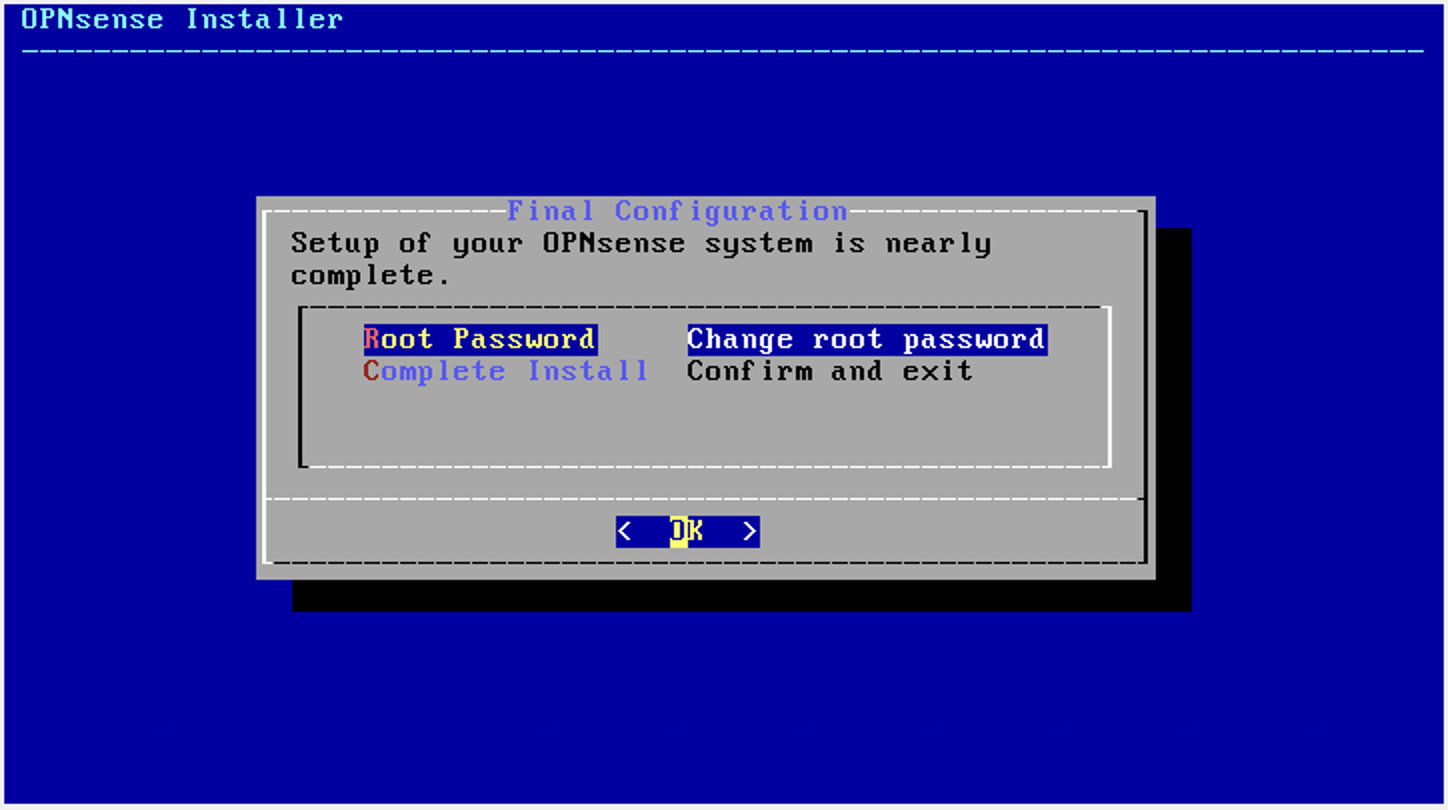
\includegraphics[width=0.9\textwidth]{2-1-1.png}
      \caption{Set Root Password}
    \end{figure}
  \item 關機後，移除 ISO 檔，重新開機。以 \texttt{root / b13901011} 登入。
\end{enumerate}

% Problem 2.2
\subsection{}
\begin{enumerate}
  \item 在 VirtualBox 設定當中，設定 Host-only Network (作為 LAN) 和 NAT Network (作為 WAN)。
    \begin{figure}[H]
      \centering
      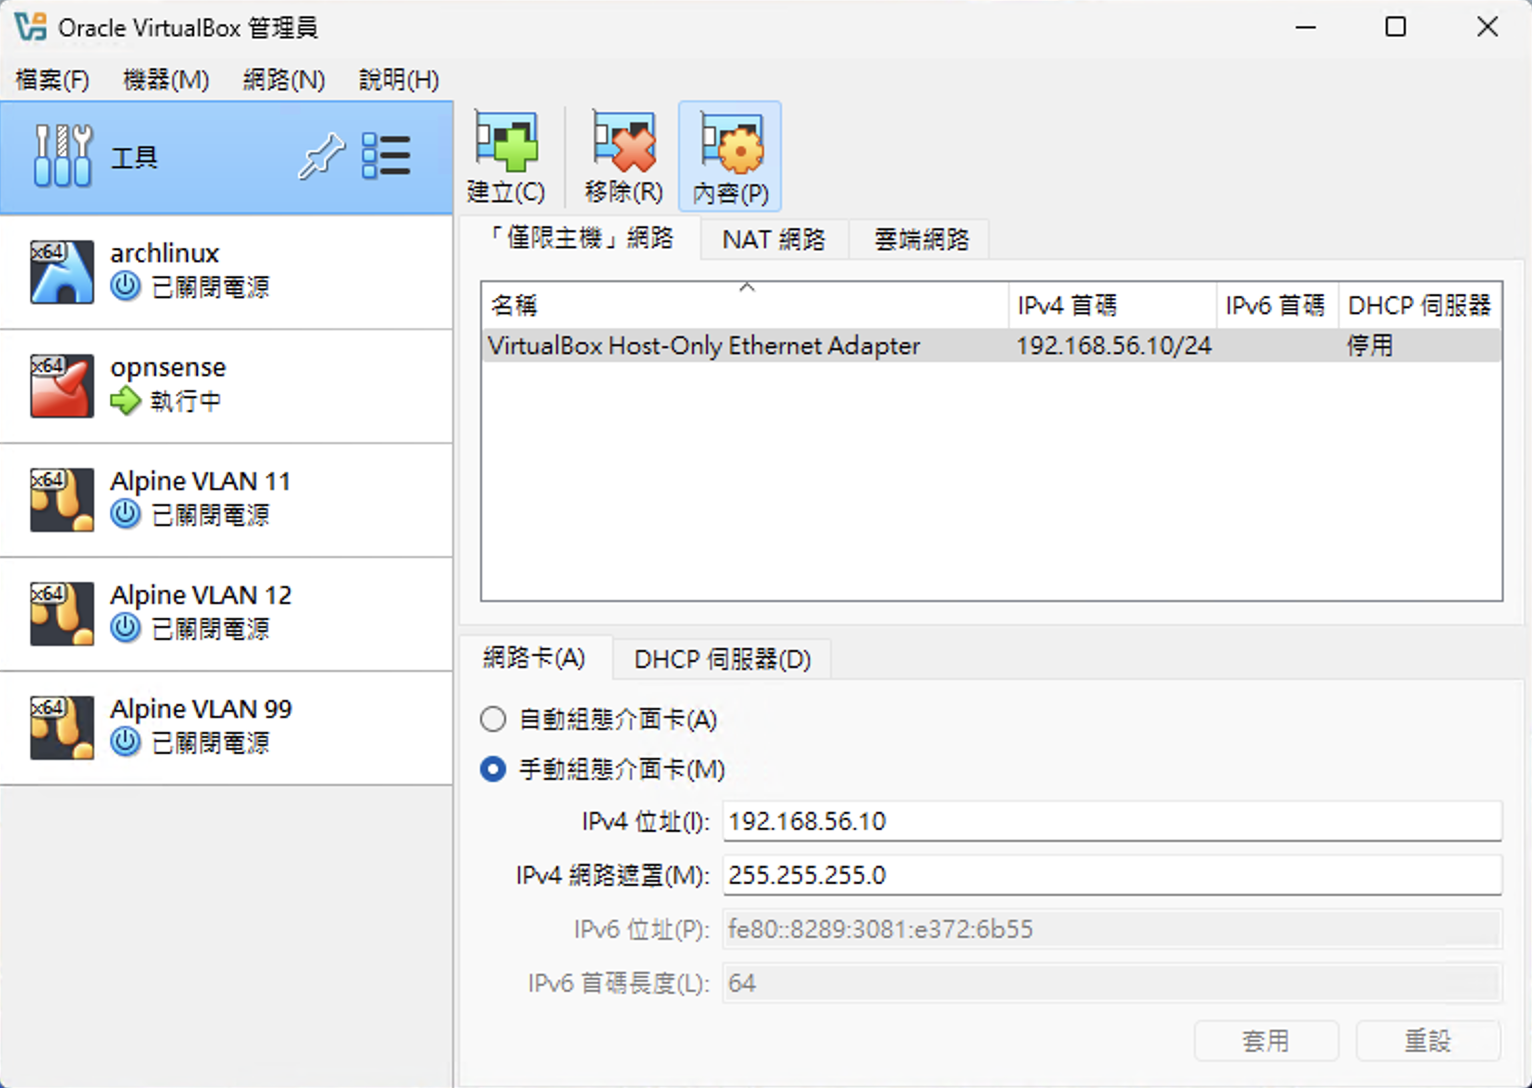
\includegraphics[width=0.49\textwidth]{2-2-1.png}
      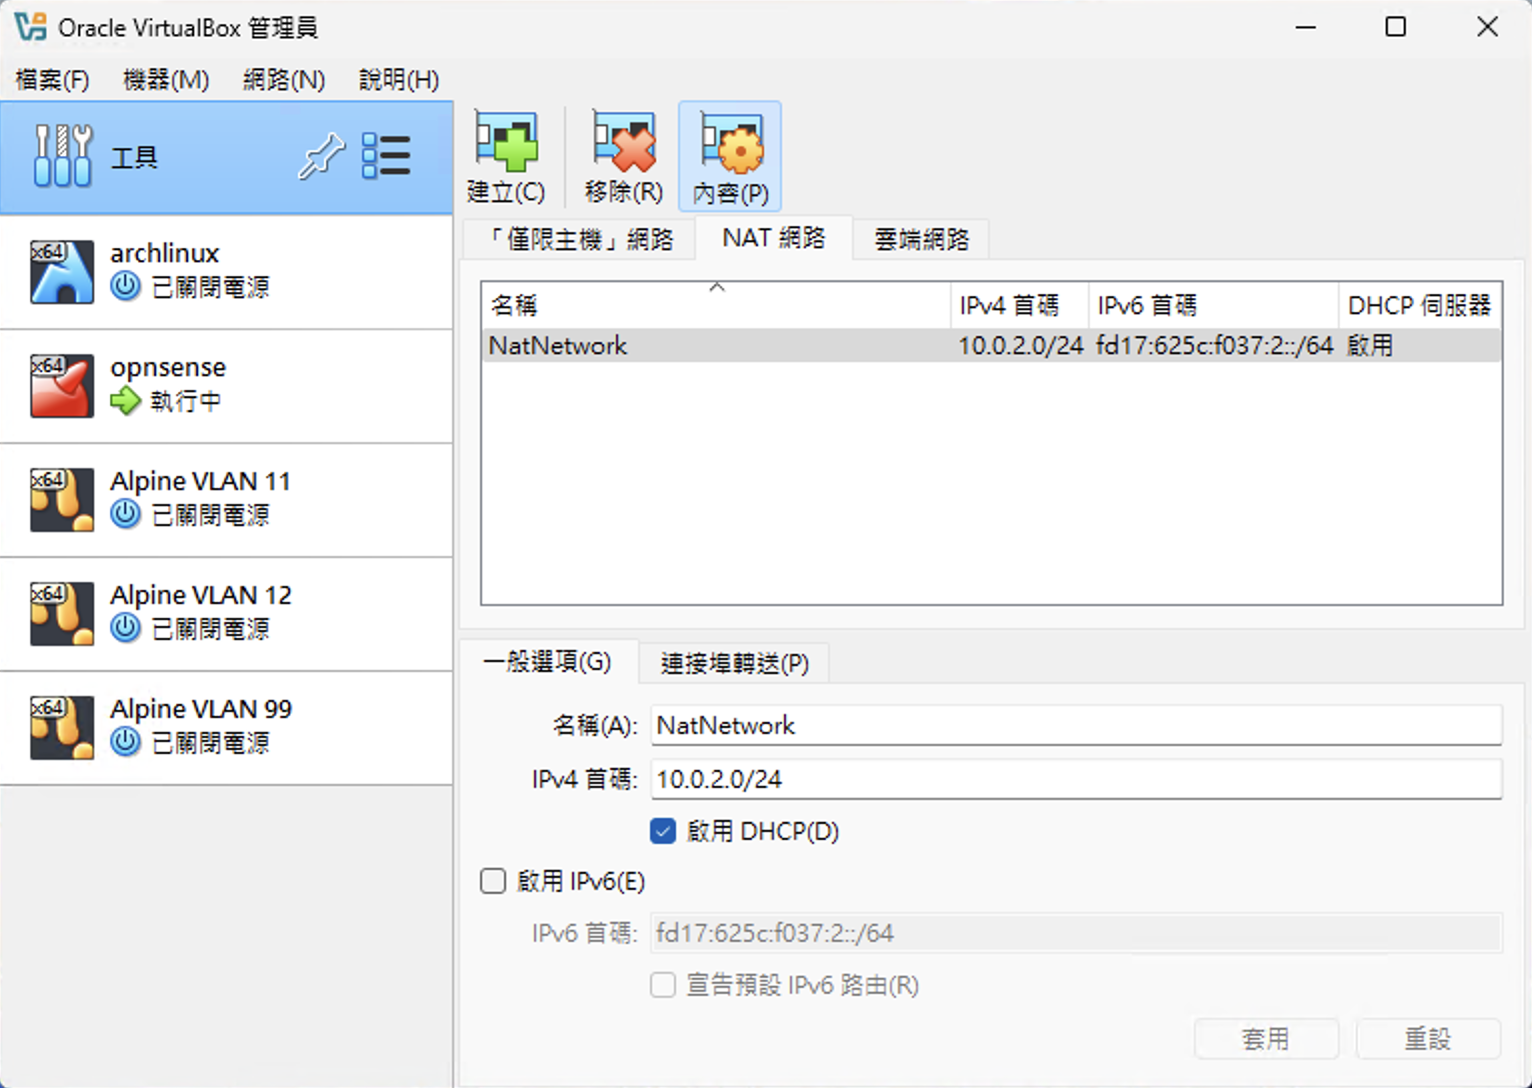
\includegraphics[width=0.49\textwidth]{2-2-2.png}
      \caption{Network Settings}
    \end{figure}
  \item 設定 OPNsense VM 的 interface:
    \begin{itemize}
      \item 按 1 進入 \texttt{Assign interfaces}，在 WAN interface 選擇 \texttt{em1}，在 LAN interface 選擇 \texttt{em0}，最後按 y 進行修改
      \item 按 2 進入，將 \texttt{1 - LAN} 的 ip address 設定為 \texttt{192.168.56.1/24}，並將 \texttt{1 - WAN} 設定為 DHCP。
    \end{itemize}
    \begin{table}[H]
      \centering
      \begin{tabular}{p{3cm}p{4cm}p{6cm}}
        \toprule
        \textbf{Interface} & \textbf{Network Type} & \textbf{IP / Subnet} \\
        \midrule
        LAN (em0) & Host-only Network & \texttt{192.168.56.1/24} \\
        WAN (em1) & NAT Network & \texttt{10.0.2.15/24} (DHCP) \\
        \bottomrule
      \end{tabular}
    \end{table}
  \item 在 Host 的 Browser 中，使用 LAN ip 進入 OPNsense 的 Web GUI，登入帳號為 \texttt{root}，密碼為 \texttt{b13901011}。
  \item 在 Setup Wizard 當中的 \texttt{Configure WAN Interface}頁面當中，取消選取 \texttt{"Block private networks from entering via WAN"} 以及 \texttt{"Block non-Internet routed networks from entering via WAN"}。
  \item 在 Interfaces > Devices > VLAN 當中，設定以下 VLAN，並按下 Apply。
    \begin{table}[H]
      \centering
      \begin{tabular}{p{2cm}p{5.5cm}p{1cm}p{3cm}p{2.5cm}}
        \toprule
        \textbf{Device} & \textbf{Parent} & \textbf{Tag} & \textbf{PCP} & \textbf{Description} \\
        \midrule
        vlan0.11 & em0 (08:00:27:9f:f1:c3)[LAN] & 11 & Best Effort (0) & VLAN 11 \\
        vlan0.12 & em0 (08:00:27:9f:f1:c3)[LAN] & 12 & Best Effort (0) & VLAN 12 \\
        vlan0.99 & em0 (08:00:27:9f:f1:c3)[LAN] & 99 & Best Effort (0) & VLAN 99 \\
        \bottomrule
      \end{tabular}
    \end{table}
  \item 在 Interface > Assignments 當中，加入三個 VLAN 的 interface。
  \item 在 Interface > [VLAN \texttt{<number>}] (\texttt{<number>} $ = {11, 12, 99}$)當中，分別 {Enable Interface}， IPv4 Configuration Type 選擇 Static IPv4，並設定防火牆 IP 位址。
    \begin{table}[H]
      \centering
      \begin{tabular}{p{3cm}p{4cm}}
        \toprule
        \textbf{VLAN} & \textbf{IPv4 Address}  \\
        \midrule
        VLAN 11 & 10.30.11.1/24 \\
        VLAN 12 & 10.30.12.1/24 \\
        VLAN 99 & 10.30.99.1/24 \\
        \bottomrule
      \end{tabular}
    \end{table}
\end{enumerate}

% Problem 2.3
\subsection{}
\begin{enumerate}
  \item Navigate to Services > ISC DHCPv4 > [VLAN 11] on the web UI.
  \item 點選 Enable DHCP server on VLAN 11。
  \item 將 Range 設為 from \texttt{10.30.11.100} to \texttt{10.30.11.199}
  \item 設定 DNS Server 為 \texttt{8.8.8.8} 和 \texttt{8.8.4.4}。
  \item 點選 Save，並且重複上述步驟設定 VLAN 12 和 VLAN 99 的 DHCP Server。
  \item 分別進入 Firewall > Rules > [VLAN 11]、[VLAN 12]、和 [VLAN 99]，並且新增規則以允許 DHCP 的封包進入。
    \begin{table}[H]
      \centering
      \begin{tabular}{llllllll}
        \toprule
        \textbf{Interface} & \textbf{Action} & \textbf{Direction} & \textbf{Protocol} & \textbf{Source} & \textbf{Port} & \textbf{Destination} & \textbf{Port} \\
        \midrule
        VLAN 11 & Pass & In & IPv4 UDP & VLAN 11 net & 68 & This Firewall & 67 \\
        VLAN 12 & Pass & In & IPv4 UDP & VLAN 11 net & 68 & This Firewall & 67 \\
        VLAN 99 & Pass & In & IPv4 UDP & VLAN 12 net & 68 & This Firewall & 67 \\
        \bottomrule
      \end{tabular}
    \end{table}
  \item 在 Firewall > Rules > WAN 中，新增以下規則以阻擋對外部發送 DHCP 封包。
    \begin{table}[H]
      \centering
      \begin{tabular}{llllllll}
        \toprule
        \textbf{Interface} & \textbf{Action} & \textbf{Direction} & \textbf{Protocol} & \textbf{Source} & \textbf{Port} & \textbf{Destination} & \textbf{Port} \\
        \midrule
        WAN & Block & Out & IPv4 UDP & This Firewall & 67 & WAN net & 68 \\
        \bottomrule
      \end{tabular}
    \end{table}
  \item Save and Apply Changes.
\end{enumerate}
\clearpage
% Problem 2.4
\subsection{}
\begin{enumerate}
  \item 進到 Firewall > Aliases 頁面。
  \item 新增以下的 Aliases:
    \begin{table}[H]
      \centering
      \begin{tabular}{p{2.5cm}p{2cm}l}
        \toprule
        \textbf{Name} & \textbf{Type} & \textbf{Content} \\
        \midrule
        \texttt{ADMIN\_PORTS} & Port(s) & 22, 80, 443 \\
        \texttt{CSIE\_WS} & Host(s) & ws1.csie.org, ws2.csie.org, ..., ws7.csie.org \\
        \texttt{GOOGLE\_DNS} & Host(s) & 8.8.8.8, 8.8.4.4 \\
        \bottomrule
      \end{tabular}
    \end{table}
    \begin{figure}[H]
      \centering
      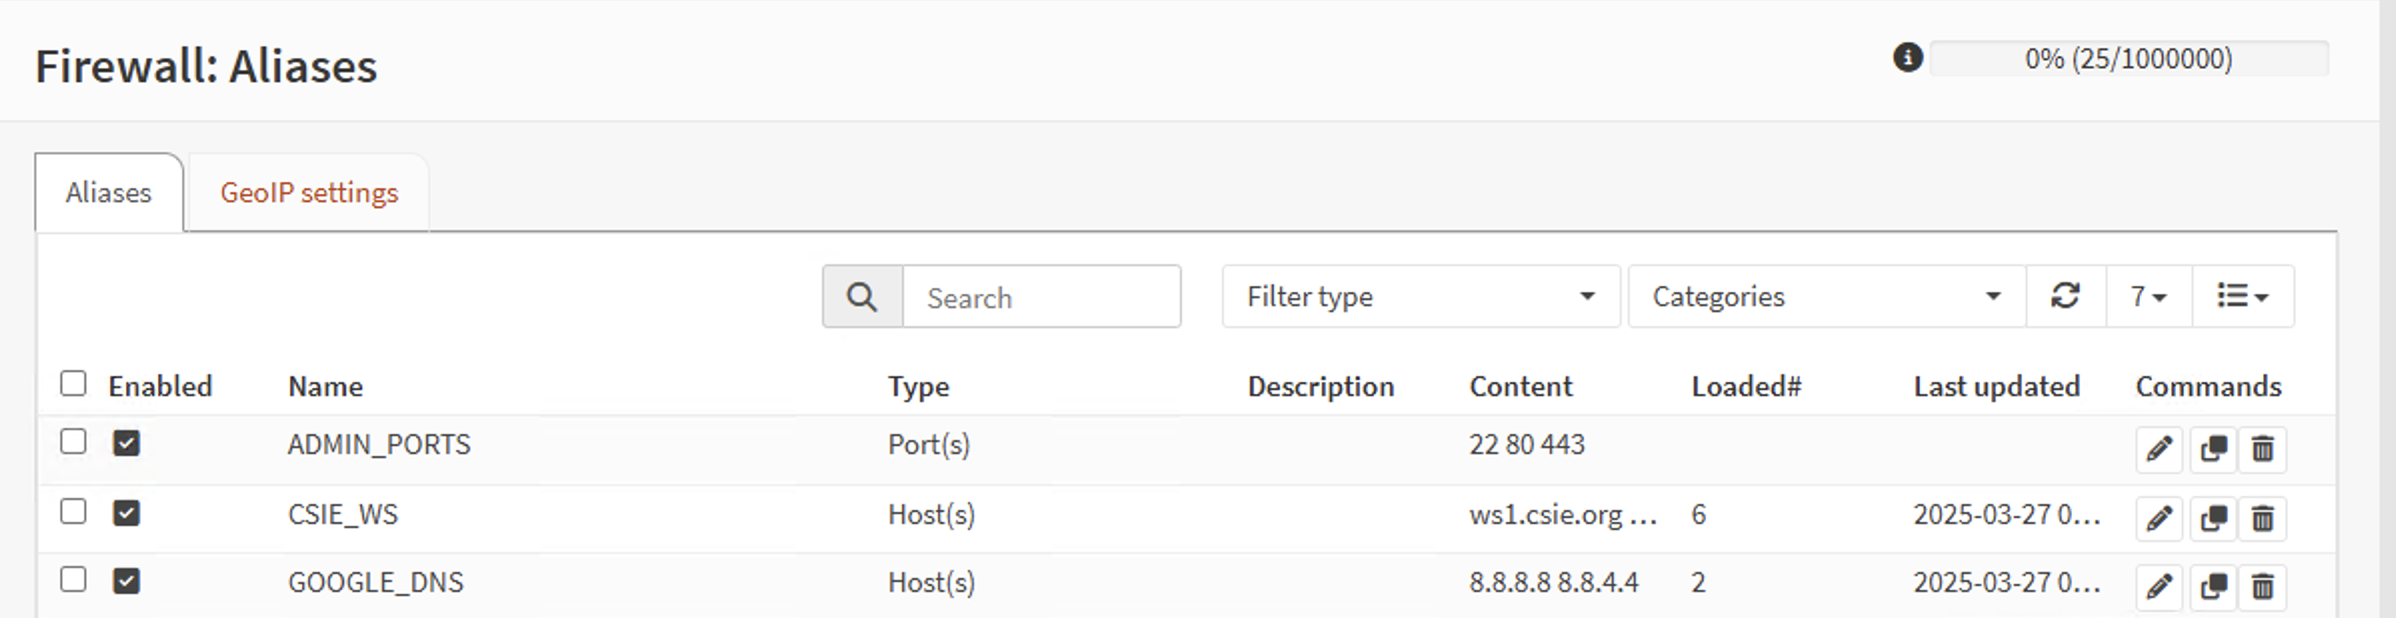
\includegraphics[width=0.9\textwidth]{2-4-1.png}
      \caption{Setup Aliases}
    \end{figure}
  \item 按下 Apply。
\end{enumerate}

% Problem 2.5
\subsection{}
\begin{enumerate}
  \item 啟用 SSH 服務。
    \begin{enumerate}
      \item 進到 Firewall > Settings > Administration 頁面。
      \item 在 Secure Shell 的區塊中，勾選 \texttt{Enable Secure Shell}、\texttt{Permit root user login} 和 \texttt{Permit password login}
      \item \texttt{Logic Group} 選擇 \texttt{wheel, admins}。
      \item \texttt{Listen Interfaces} 選擇 \texttt{VLAN 99}。
      \item 按下 Save。
    \end{enumerate}
  \item 設定規則
    \begin{enumerate}
      \item 進入 Firewall > Rules > [VLAN 99] 頁面。
      \item 新增以下規則，分別允許 VLAN 99 連線到防火牆的 \texttt{ADMIN\_PORTS} 和 \texttt{GOOGLE\_DNS}、\texttt{CSIE\_WS}。
        \begin{table}[H]
          \centering
          \small
          \begin{tabular}{lllllll}
            \toprule
            \textbf{Action} & \textbf{Direction} & \textbf{Protocol} & \textbf{Source} & \textbf{Port} & \textbf{Destination} & \textbf{Port} \\
            \midrule
            Pass & In & IPv4 TCP/UDP & \texttt{VLAN99 net} & * & \texttt{\footnotesize This Firewall} & \texttt{\footnotesize ADMIN\_PORTS} \\
            Pass & In & IPv4 * & \texttt{VLAN99 net} & * & \texttt{\footnotesize CSIE\_WS, GOOGLE\_DNS} & * \\
            \bottomrule
          \end{tabular}
        \end{table}
    \end{enumerate}
  \item 按照 Lab 5 簡報當中的方式，架設一台 Alpine Linux VM，並且透過 DHCP 獲得 VLAN 99 的 IP。我連線到 NTU VPN，並獲取以下結果截圖：
    \begin{figure}[H]
      \centering
      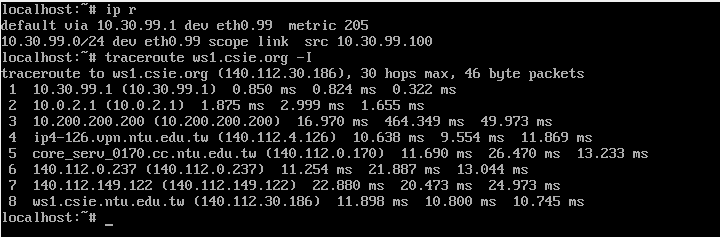
\includegraphics[width=0.88\textwidth]{2-5-1.png}
      \caption{Screenshot of \texttt{ip r} and \texttt{traceroute}}
    \end{figure}
    \vspace{-0.6cm}
    \begin{figure}[H]
      \centering
      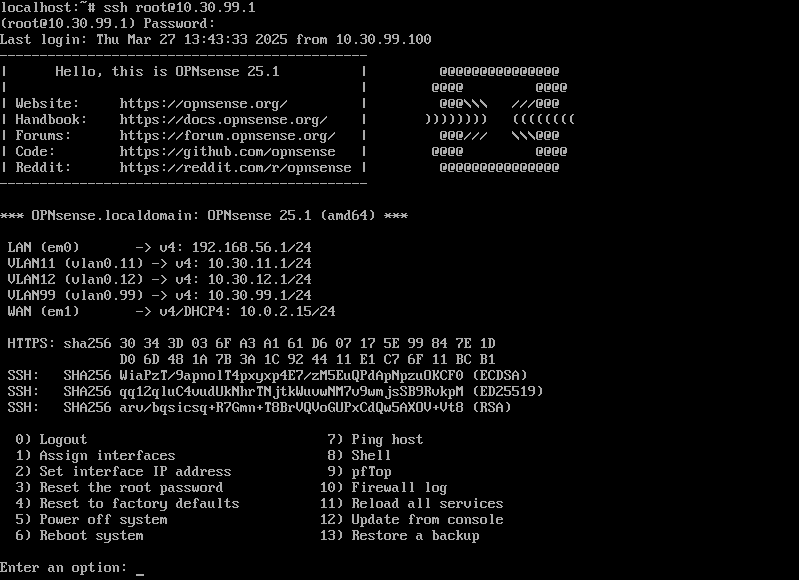
\includegraphics[width=0.88\textwidth]{2-5-2.png}
      \caption{Screenshot of SSH to OPNsense Firewall}
    \end{figure}
    \vspace{-1cm}
\end{enumerate}

% Problem 2.6
\subsection{}
\begin{enumerate}
  \item 進到 System > Aliases 頁面，並新增一個 Alias 來阻擋特定列表的 IP 位址。
    \begin{table}[H]
      \centering
      \begin{tabular}{p{2.5cm}lll}
        \toprule
        \textbf{Name} & \textbf{Type} & \textbf{Refresh Frequency}  & \textbf{Content} \\
        \midrule
        \texttt{BLOCK\_LIST} & URL Table (IPs)& 1 Day & 題目給的網址\\
        \bottomrule
      \end{tabular}
    \end{table}
  \item 在 Firewall > Settings > Schedules 頁面，新增一個 Schedules。Description 欄位設定為 \texttt{monday\_mornings}，在 Month 欄位下方的日曆當中，按下 Mon 來選擇所有週一。Time 欄位中，選擇 Start Time 為 9:00，end time 為 12:00，並按下 Add Time。最後按下 Save。
    \begin{figure}[H]
      \centering
      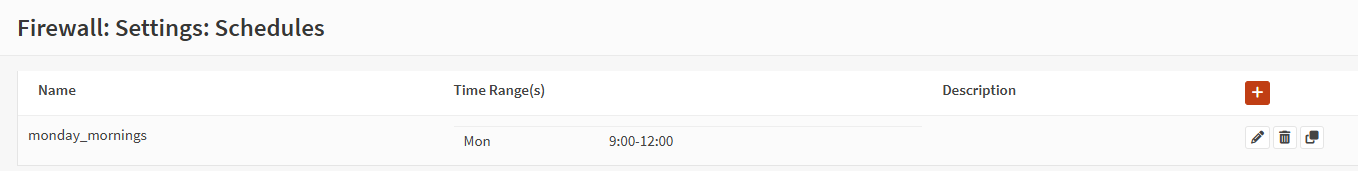
\includegraphics[width=\textwidth]{2-6-1.png}
      \caption{Setup Schedule}
    \end{figure}
  \item 在 Firewall > Rules > VLAN11 頁面，依序新增以下規則（加在 Problem 2.3 的規則後）：
    \begin{table}[H]
      \centering
      \small
      \begin{tabular}{llllllll}
        \toprule
        \textbf{Action} & \textbf{Direction} & \textbf{Protocol} & \textbf{Source} & \textbf{Port} & \textbf{Destination} & \textbf{Port} & \textbf{Schedule} \\
        \midrule
        Block & In & IPv4 * & \texttt{VLAN11 net} & * & * & * & \texttt{monday\_mornings} \\
        Block & In & IPv4 * & \texttt{VLAN11 net} & * & \texttt{VLAN99 net} & * & * \\
        Block & In & IPv4 * & \texttt{VLAN11 net} & * & \texttt{This Firewall} & * & * \\
        Block & In & IPv4 * & \texttt{VLAN11 net} & * & \texttt{BLOCK\_LIST} & * & * \\
        Pass & In & IPv4 * & \texttt{VLAN11 net} & * & * & * & * \\
        \bottomrule
      \end{tabular}
    \end{table}

  \item 在 Firewall > Rules > VLAN12 頁面，依序新增以下規則（加在 Problem 2.3 的規則後）：
    \begin{table}[H]
      \centering
      \small
      \begin{tabular}{llllllll}
        \toprule
        \textbf{Action} & \textbf{Direction} & \textbf{Protocol} & \textbf{Source} & \textbf{Port} & \textbf{Destination} & \textbf{Port} & \textbf{Schedule} \\
        \midrule
        Block & In & IPv4 * & \texttt{VLAN12 net} & * & * & * & \texttt{monday\_mornings} \\
        Block & In & IPv4 * & \texttt{VLAN12 net} & * & \texttt{VLAN99 net} & * & * \\
        Block & In & IPv4 * & \texttt{VLAN12 net} & * & \texttt{This Firewall} & * & * \\
        Block & In & IPv4 * & \texttt{VLAN12 net} & * & \texttt{BLOCK\_LIST} & * & * \\
        Block & In & IPv4 * & \texttt{VLAN12 net} & * & \texttt{VLAN11 net} & * & * \\
        Pass & In & IPv4 * & \texttt{VLAN12 net} & * & * & * & * \\
        \bottomrule
      \end{tabular}
    \end{table}
  \item Apply Changes.
\end{enumerate}
% Problem 2.7
\subsection{}
按照題目所敘，到 \texttt{System > Configuration > Backups} 頁面，點選 Download Configuration 即可。

% -----------------------------------------------------------
%    You don't have to mess with anything below this line.
% -----------------------------------------------------------

\end{document}
